\section{An Overview of NMR Data Analysis}
To gain insights from \ac{NMR} experiments on the chemical system of interest,
extraction of the defining parameters $\bth$ is necessary, though the majority
of \ac{NMR} users are unlikely to think about the process of \ac{NMR} analysis
in this way. For example:
\begin{itemize}
    \item An understanding of the chemical environments of atoms in a molecule
        can be gained by considering the chemical shifts of the various peaks
        in the spectra, which are a proxy for the \ac{FID} frequencies
        $\symbf{f}$.
    \item  The relative stoichiometries\note{does this make sense?} of a
        molecule can be elucidated by inspecting the integrals of spectral
        peaks, which are directly related to the \ac{FID} amplitudes $\bda$
\end{itemize}

\note{
    \begin{itemize}
        \item Typical approach to analysing the data (FT, peak pick, integrate, baseline correction, window functions, zero-filling etc),
        \item Estimation techniques: LP, SVD techniques, iterative techniques (AMARES, VARPRO), Bayesian techniques (CRAFT), ML techniques
    \end{itemize}
}

\subsection{Conventional NMR Analysis}
The conventional route to interpret \ac{NMR} experiments is to
transform the raw output (the \ac{FID}) into the frequency domain, producing an
\ac{NMR} spectrum. This is achieved through application of the \acf{FT}:
\begin{subequations}
    \begin{flalign}
        &\text{Continuous case:} &&\FT( x(t) )(f) =  \int_{-\infty}^{\infty} x(t) \exp \left(
            -2 \pi \iu t f \right) \mathrm{d} t
            \quad \forall t \in \mathbb{R},\\
        &\text{Discrete case:} &&\FT( \symbf{x} )[n] =  \sum_{k=0}^{N-1} \symbf{x}[k] \exp \left(
            -\frac{2 \pi \iu k n}{N} \right)
            \quad \forall n \in \lbrace 0, \cdots, N-1 \rbrace.
    \end{flalign}
\end{subequations}
The \ac{FT} of a single exponentially-damped complex sinusoid takes the form of
a Lorentzian\footnote{
    For the discrete case, an upshot of only possessing data for $t > 0$ is
    that the \ac{FT} of an \ac{FID} features a vertical offset,
    such that the baseline does not sit at 0\cite{Tang1994}. This is corrected
    by halving the initial point of the \ac{FID} prior to \ac{FT}.
}:
\begin{subequations}
    \begin{gather}
        s(f) = \FT\left(
            a \exp(\iu \phi) \exp\left(\left(\iu \Updelta f - \etaone\right) t\right) \right) (f),\\
        s(f) = \frac{a \exp(\iu \phi) }
            {\etaone + \iu \Updelta f},\\
        \Updelta f = 2 \pi \left(\fone - \foffone - f \right).
    \end{gather}
\end{subequations}
When $a = \phi = 0$, this function is equivalent to the (unnormalised) \ac{pdf}
of the Cauchy distribution. The \ac{FT} is a linear function, such that the
\ac{FT} of a summation of signals is equivalent to the summation of the
\acp{FT} of each signal. A corollary is that an \ac{NMR} spectrum comprises a
series of Lorentzian ``peaks'', located at the resonance frequencies of
detected
coherences:
\begin{equation}
    s(f) = \sum_{m=0}^{M-1}
    \frac{\bdam \exp(\iu \bdphim)}
    {\bdetaone + \iu \Updelta f_m}.
    \label{eq:ft-summation}
\end{equation}
The \ac{FT} is a very attractive means of processing \ac{NMR} data, as it
presents the data in a format which is human-interpretable, with the basic
rules describing how chemical structure is mapped to \ac{NMR} spectral
properties being a fundamental skill that virtually all experimental chemists
require\cite{Hore2015b}. Due to innate properties of the \ac{NMR} experiment,
as well as features arising from analysing a discrete signal, the raw output
from an \ac{NMR} experiment often leads to spectra with undesirable
characteristics without any extra manipulation. An outline of extra processing
steps that are frequently applied to \ac{NMR} data are now presented.

\subsubsection{Apodisation}
Apodisation refers to the process of mutating a signal by multiplying it with a
specified function, often called a \emph{window function}. Apodisation is frequently used for the purposes of either \emph{sensitivity enhancement} or \emph{resolution enhancement}.

\paragraph{Sensitivity Enhancement} As \iac{FID} progresses with time, the
contributions from the desirable signal and experimental noise becomes more
weighted towards the noise, as spin relaxation phenomena dampen the signal. As
such, multiplying the \ac{FID} with a function which is initially large, and
gets progressively smaller with time can be used to enhance the sensitivity
(i.e. the \ac{SNR}) of the \ac{FID}. The most common function to achieve this
is the negative exponential such that a given point is multiplied by $\exp(-k
\none)$. While this enhances sensitivity, application of this window function
also has the undesirable effect of broadening the spectral peaks, which can
make the spectrum harder to interpret, especially when resonances with similar
frequencies exist.

\paragraph{Resolution Enhancement} The resolving power of a spectrum is largely
dictate by the broadness of the contributing peaks, which is directly related
to the rate of damping associated with the contributing oscillators in the
\ac{FID}. Resolution enhancement can be achieved by applying a window function
that artificially reduced the rate of oscillator decay, by suppressing points
that are early in the \ac{FID}. Popular examples of window functions for
resolution enhancement are the Lorentz-Gauss function, which bestow a sharper,
Gaussian shape to the peaks, and the sine-bell, which is commonly used in
multidimensional experiments. All window functions reduce the sensitivity of
the resulting spectra, since initial points, where the desirable signal is at
its greatest intensity, are attenuated.

By being defined to decay to $0$ at the end of the \ac{FID}, window functions
are also able to suppress \emph{truncation artefacts}, which appear when the
\ac{FID} still possesses appreciable signal amplitude at the end of the
acquisition period. Truncated \acp{FID} lead to peaks with a form that is akin
to the convolution of the \ac{FT} of the untruncated \ac{FID}, with the
\ac{FT} of a box-function, which takes the form $\nicefrac{sin(x)}{x}$.

\subsubsection{Phase correction}
The real and imaginary components of \eqref{eq:ft-summation} are as follows:
\begin{subequations}
    \begin{gather}
        \Re(s(f)) = \sum_m
        \frac{\bdam \left(\cos(\bdphim) \bdetaonem + \sin(\bdphim) \Updelta f_m\right)}
        {\bdetaonem^2 + \left( \Updelta f_m \right)^2},\\
        \Im(s(f)) = \sum_m
        \frac{\bdam \left(\sin(\bdphim) \bdetaonem - \cos(\bdphim) \Updelta f_m\right)}
        {\bdetaonem^2 + \left( \Updelta f_m \right)^2}.
    \end{gather}
\end{subequations}
If all oscillators have a phase of \ang{0}, the above expressions simplify to
\begin{subequations}
    \begin{gather}
        \Re(s(f)) = \sum_m
        \frac{\bdam \bdetaonem}
        {\bdetaonem^2 + \left( \Updelta f_m \right)^2},
        \label{eq:absorption}\\
        \Im(s(f)) = -\sum_m
        \frac{\bdam \Updelta f_m}
        {\bdetaonem^2 + \left( \Updelta f_m \right)^2}.
        \label{eq:dispersion}
    \end{gather}
\end{subequations}
Peaks of the form in \eqref{eq:absorption} are \emph{absorption} Lorentzians,
while those of the form in \eqref{eq:dispersion} are \emph{dispersion}
Lorentzians. As illustrated clearly in panel c2 of Figure
\ref{fig:amp-phase-freq-damp}, a peak with an absorption lineshape is far more
desirable than a dispersion one for two key reasons: (i) its maximum
corresponds to the oscillator frequency, while a dispersion Lorentzian
has a magnitude of $0$ at the oscillator frequency (ii) they decay more rapidly
towards $0$. Generating a spectrum where all peaks possess absorption
Lorentzians is therefore desired. Fortunately, for the majority of \ac{NMR} experiments\footnote{
    An example of an exception to this rule is the use of a frequency-swept, or
    ``chirped'' pulse, which generate datasets with quadratic phase behaviour.
    \note{refer to
    BBQCHILI section when written up}.
}, the phases of the contributing resonances possess a phase which depends
linearly (to first-order) on their frequency, i.e.
\begin{equation}
    \bdphim = \phi_0 + \phi_1 \bdfonem,
\end{equation}
where $\phi_0, \in (-\pi, \pi]$ and $\phi_1 \in \mathbb{R}$ are zero- and
first-order phase terms. A feature of all \ac{NMR} processing platforms is the
ability to perform phase-correction, in which the user effectively determines
$\phi_0$ and $\phi_1$ by inspecting the appearance of the spectrum for
different values of $p_0$ and  $p_1$, according to
\begin{equation}
    \symbf{s}_{\phi} \left[\none\right] =
    \symbf{s} \left[\none\right]
    \exp\left(\iu \left(p_0 + \frac{p_1 \none}{\None}\right)\right),
\end{equation}
in an attempt to give all peaks in the spectrum absorption-mode lineshapes. The
optimal values of $p_0$ and  $p_1$ are $-\phi_0$ and  $-\phi_1$, respectively.

\subsubsection{Baseline correction}
\cite{Cobas2006}

\begin{figure}
    \centering
    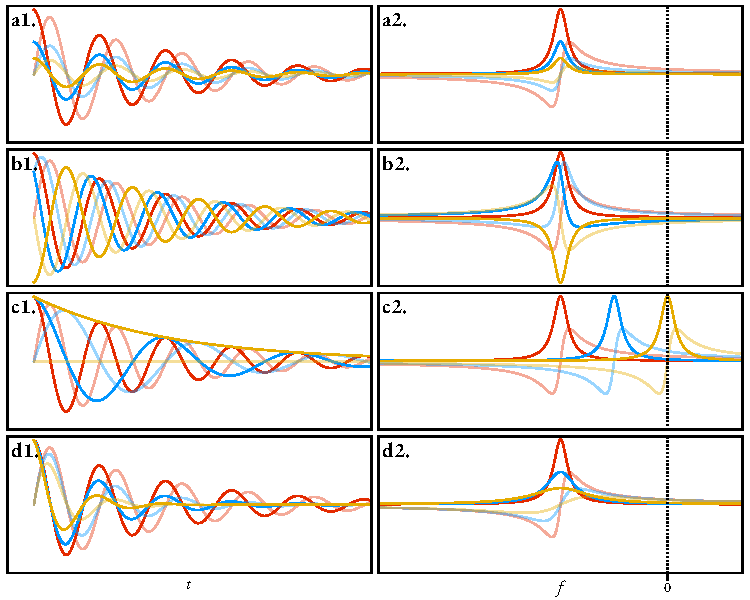
\includegraphics{amp_phase_freq_damp/amp_phase_freq_damp.pdf}
    \caption{An illustration of the influence of the four parameters associated
        with an oscillator in both the time-domain (panels \textbf{a1.} -- \textbf{d1.}) and Fourier-domain
        (panels \textbf{a2.} -- \textbf{d2.}). The red
        signal is generated with the same parameters across all panels:
        $a = a_{\text{red}}$, $\phi = 0$, $f = f_{\text{red}}$,  $\eta =
        \eta_{\text{red}}$.
        The blue and yellow signals were produced by altering one parameter out of the four.
        \textbf{a.}
        $a_{\text{blue}} = \nicefrac{1}{2} a_{\text{red}}$,
        $a_{\text{yellow}} = \nicefrac{1}{4} a_{\text{red}}$.
        \textbf{b.}
        $\phi_{\text{blue}} = \nicefrac{\pi}{4}$,
        $\phi_{\text{yellow}} = \pi$.
        \textbf{c.}
        $f_{\text{blue}} = \nicefrac{1}{2} f_{\text{red}}$,
        $f_{\text{yellow}} = 0$.
        \textbf{d.}
        $\eta_{\text{blue}} = \nicefrac{1}{2}\eta_{\text{red}}$,
        $\eta_{\text{yellow}} = \nicefrac{1}{4}\eta_{\text{red}}$.
        The real and imaginary components of each signal are plotted, with the
        imaginary component being paler than its real counterpart.
    }
    \label{fig:amp-phase-freq-damp}
\end{figure}
\subsection{Estimation Techniques for NMR Analysis}
